%  LaTeX support: latex@mdpi.com 
%  For support, please attach all files needed for compiling as well as the log file, and specify your operating system, LaTeX version, and LaTeX editor.

%=================================================================
\documentclass[universe,article,submit,pdftex,moreauthors]{Definitions/mdpi} 
\usepackage{amsmath}


%=================================================================
% MDPI internal commands - do not modify
\firstpage{1} 
\makeatletter 
\setcounter{page}{\@firstpage} 
\makeatother
\pubvolume{1}
\issuenum{1}
\articlenumber{0}
\pubyear{2025}
\copyrightyear{2025}
%\externaleditor{Firstname Lastname} % More than 1 editor, please add `` and '' before the last editor name
\datereceived{ } 
\daterevised{ } % Comment out if no revised date
\dateaccepted{ } 
\datepublished{ } 
%\datecorrected{} % For corrected papers: "Corrected: XXX" date in the original paper.
%\dateretracted{} % For retracted papers: "Retracted: XXX" date in the original paper.
\hreflink{https://doi.org/} % If needed use \linebreak

%=================================================================
% Full title of the paper (Capitalized)
\Title{Emergent Cosmology from Quasicrystal Growth: A Derived 5/6 Scaling Law}
\TitleCitation{Emergent Cosmology from Quasicrystal Growth}

% Author Orchid ID: enter ID or remove command
%\newcommand{\orcidauthorA}{0000-0002-0637-1916} % Add \orcidA{} behind the author's name
%\newcommand{\orcidauthorB}{0000-0002-3411-4394} % Add \orcidB{} behind the author's name

% Authors, for the paper (add full first names)
%\Author{Marcelo Amaral $^{1}$*\orcidauthorA{}, Yadav Aman $^{2}$\orcidauthorA{}}
\Author{Marcelo Maciel Amaral $^{1}$*, Aman Yadav $^{2}$}

%\longauthorlist{yes}

% MDPI internal command: Authors, for metadata in PDF
\AuthorNames{Marcelo Maciel Amaral, Aman Yadav}


\isAPAStyle{%
         \AuthorCitation{Maciel Amaral, M., \& Yadav, A.}
    }{%
         \isChicagoStyle{%
         \AuthorCitation{Maciel Amaral, Marcelo, and Aman Yadav}
    }{
         \AuthorCitation{Maciel Amaral, M.; Yadav, A.}
    }
}

% Affiliations / Addresses (Add [1] after \address if there is only one affiliation.)
\address{%

$^{1}$ \quad Gauge Freedom, Inc.,
Los Angeles, CA, USA; Marcelo@GaugeFreedom.com\\
$^{2}$ \quad Delhi Technological University,
Rohini, 110042, Delhi, India; amanyadaav11@gmail.com}
% Contact information of the corresponding author
\corres{Corresponding author}


\abstract{We model spacetime as a growing quasicrystal generated by shell-by-shell projection of the $E_8$ lattice. Under few geometric assumptions and without cosmological parameter fits, we derive the parameter-free scaling $a(n)\asymp n^{5/6}$ for the emergent scale factor, where $n$ is the discrete growth step. The law follows from lattice combinatorics and outer-scale growth, fixing the exponent independently of cosmology. We define $a(n)$ via a typical spacing (quantile $k$-nearest-neighbor) and show that large-scale simulations exhibit the predicted power-law envelope with characteristic staircase behavior due to discrete shell injections. Further, introducing a physical ``growth clock'' $\dot n=\kappa n^\alpha$ yields $a(t)\propto t^{\frac{5}{6(1-\alpha)}}$ and the correspondence $w(\alpha)=-(1+4\alpha)/5$, linking microscopic growth kinetics to FLRW eras. The framework acknowledges warm-inflation dynamics with dissipative reheating, offers a phonon dark matter candidate, and suggests a kinetic pathway relevant to the Hubble-tension puzzle.}


% Keywords
\keyword{Quantum Gravity; Cosmology; Hubble Tension; Quasicrystals} 


%%%%%%%%%%%%%%%%%%%%%%%%%%%%%%%%%%%%%%%%%%
\begin{document}
\section{Introduction}

Recent work across quantum gravity and cosmology has sharpened a viewpoint in which spacetime and gravity are effective, emergent descriptions governed by symmetry, coarse-graining, and renormalization-group flow rather than fixed microscopic assumptions \cite{Verlinde2011}. From this viewpoint, prospective UV completions that are ranging from loop-based to string-inspired frameworks are assessed by their ability to recover robust infrared structures and symmetries in their long-wavelength limits, mirroring the emergence of elasticity from microscopic constituents in condensed matter systems. \cite{Rovelli-Vidotto-Book,stringbook1,Tahim2009}. Meanwhile, persistent observational puzzles most notably the Hubble tension signal that our standard cosmological model may be missing scale-dependent physics or effective interactions across epochs \cite{hubbletension,hubble,lawsofnature,Kuzmichev}. These considerations motivate approaches that foreground scale invariance, universality, and geometric/combinatorial mechanisms capable of producing cosmological dynamics without tuning.

In previous work \cite{Amaral2024}, we introduced a heuristic model motivated by these challenges, exploring a conceptual analogy between quantum mechanics in an expanding domain and Friedmann cosmology. While that work established a rationale for investigating quasicrystalline spacetime, it relied on an imposed connection between quantum and cosmological scales. In this paper, we replace that heuristic argument with a rigorous, first-principles framework. We demonstrate that the essential features of cosmic expansion emerge directly and quantitatively from the combinatorial geometry of a growing quasicrystal.

Our central result is a parameter-free derivation of the cosmological scale factor, $a(n)$, from the shell-by-shell growth of a quasicrystal projected from the 8-dimensional $E_8$ lattice. We show from lattice combinatorics alone that the scale factor follows a universal scaling law, $a(n) \asymp n^{5/6}$, where $n$ is the discrete growth step. This theoretical prediction is then validated by large-scale numerical simulations, which precisely measure the scaling exponent while also revealing a characteristic ``staircase'' growth pattern at finite scales. By introducing a physically motivated ``growth clock'' to map discrete steps to cosmic time, we derive an expansion history, $a(t)$, that reproduces all standard Friedmann--Lema\^{\i}tre--Robertson--Walker (FLRW) cosmological eras.

This framework provides a novel, geometric perspective on some of cosmology's most pressing questions. In the subsequent sections, we develop the mathematical foundations of this model, present the analytical derivation and numerical validation of the scaling law, and explore the phenomenological implications for warm inflation, dark matter, and the Hubble tension.

%%%%%%%%%%%%%%%%%%%%%%%%%%%%%%%%%%%%%%%%%%
\section{A Quasicrystalline Model of the Universe}
\label{sec:QCuniverse}

We model spacetime as a growing quasicrystal whose properties make it a natural template for cosmology. Our framework is built on a direct, computationally explicit growth mechanism: a full shell-by-shell linear projection of the 8-dimensional $E_8$ lattice. We place the origin at an $E_8$ vertex and consider the concentric shells of points, $\mathcal{S}_k$, radiating outwards. The number of points on the $n$-th shell is given by the divisor function \cite{ConwaySloane1988}:
\begin{equation}
    N_{E_8}(n)=240\,\sigma_{3}(n), \quad \text{where} \quad \sigma_{3}(n)=\sum_{d\mid n} d^{3}. \label{eq:NE8}
\end{equation}
At each discrete growth step $n$, we project the cumulative set of points from the first $n$ shells, $S(n):=\bigcup_{k\le n}\mathcal S_k$, into a 4D physical space, via a fixed rank-4 linear map, $\Pi$, yielding the point set $X(n):=\Pi\big(S(n)\big)$. A key step is that we then renormalize the entire structure by the inverse of the current minimal point spacing, $s(n):=\ell_{\min}(n)^{-1}$, to produce a final configuration $X^{\star}(n):=s(n)\,X(n)$ where the shortest distance is fixed to unity. This full-projection with renormalization scheme ensures the point sets are uniformly discrete and is the foundation for deriving the scale factor in Section~\ref{sec:QC-expansion}.

This growth process exhibits a crucial dual nature: an external expansion in overall size is accompanied by an internal subdivision, where new points are inserted within the existing volume. This dual mechanism of ``expansion + subdivision'' is the microscopic engine for the emergent cosmology we develop.

The physical consequences of this model can be understood from three complementary perspectives. At the quantum level, the growth corresponds to an evolving state within a growing Hilbert space of admissible tiling configurations \cite{Connes}. From a statistical mechanics viewpoint, the combinatorics of these tiling configurations possess an information entropy that defines an emergent energy density, which can be shown to scale as pressureless matter ($\rho \propto a^{-3}$) once the injection of new points from the higher dimension ceases \cite{Amaral2024}. Finally, at large continuum scales, the quasicrystalline structure supports collective excitations: vibrational phonons and rearrangement modes known as phasons. The low-energy dynamics of these fields are captured by an Effective Field Theory (EFT) \cite{Baggioli:2020haa}. Within this EFT, phonons behave as conventional propagating modes with a nearly relativistic dispersion, while phasons are inherently dissipative, with a characteristic dispersion relation $\omega^2 + i\,\gamma\,\omega = v^2 k^2$. This distinction is crucial for their respective cosmological roles discussed in Section~\ref{sec:pheno}.

This multi-faceted model is grounded in a precise geometric construction that provides the foundation for deriving the emergent cosmological expansion from first principles, which we now present.


\section{Emergent Cosmology from Quasicrystal Growth}
\label{sec:QC-expansion}

In the preceding section, we mentioned a heuristic model of the universe as a growing quasicrystalline structure. We now demonstrate more concretely that the large-scale cosmic expansion, typically described by the FLRW metric, arises as a natural endogenous consequence of this growth. The expansion law can be derived directly from the combinatorial and geometric properties of the underlying lattice projection, without imposing external cosmological principles at microscopic scales.

\subsection{The Physical Mechanism of Growth: Subdivision and Rescaling}

The quasicrystalline universe model incorporates two key growth mechanisms:

\paragraph{\textbf{External Growth by Shell Projection}}

The universe expands externally through the projection of new points from a higher-dimensional lattice onto our observable space. Specifically, we consider the projection of the 8-dimensional $E_8$ lattice via a fixed rank–4 linear map $\Pi:\mathbb{R}^8\!\to\!\mathbb{R}^4$ (Elser–Sloane geometry), and visualize on a generic 3D slice.
This process adds concentric shells of points, effectively growing the quasicrystal universe shell by shell.

\paragraph{\textbf{Internal Growth through Subdivision and Rescaling}}

As new points are projected, they may appear within existing structures, leading to internal subdivision. Due to the quasicrystal's self-similarity, the tile structures are preserved at different scales. To compare stages at a fixed microscopic resolution, we apply a global renormalization by the current minimal spacing; whenever new points introduce a smaller spacing, all distances are rescaled so that the nearest–neighbor length remains fixed (our unit).

The mechanism is transparent in lower-dimensional quasicrystals examples, such as the Fibonacci chain (one-dimensional) and the Penrose tiling (two-dimensional), which can be built with just two tile types. Steinhardt's one-tile quasicrystal~\cite{Steinhardt1996} further demonstrates how tiles keep dividing but reappear at different scales due to self-similarity. In three dimensions, quasicrystals like the 3D Penrose tiling involve more complex arrangements but follow the same principle~\cite{Duneau1985}. In four dimensions, with the Elser-Sloane Quasicrystals, the number of tiles is not well known, but the building block is the 600-cell polytope, which keeps arising at different scales.

To verify the scaling behavior of this growth mechanism directly, we performed a large-scale numerical simulation.

\subsection{Numerical Validation of the Scaling Law}

We simulated full shell-by-shell projection of the $E_8$ lattice up to $n=18$, generating the cumulative point set $X(n)$ at each step (final size $>5\times10^6$ points). For each $X(n)$ we computed a robust typical spacing
\[
\ell_q(n):=\mathrm{median}\{\text{1st-nearest-neighbor distance}\},
\]
and defined the emergent scale factor $a(n):=\ell_q(1)/\ell_q(n)$. By construction $\ell_q(n)$ tracks the density proxy $\ell_{\mathrm{typ}}(n)=(V/M)^{1/3}$ up to an $O(1)$ factor, so $a(n)$ probes the same asymptotic exponent.

The measured $a(n)$ (Fig.~\ref{fig:numerical_scaling}) exhibits a staircase: long plateaus punctuated by abrupt increases when newly injected shells create denser local configurations. Because plateaus bias log–log regressions, we identify the ``jump points'' (the $n$ at which $a(n)$ increases) and fit only these to recover the envelope of the growth. A log–log fit to the 8 jump points observed up to $n=18$ yields a slope $\hat\gamma_{\mathrm{env}}=0.743$. This is consistent with the theoretical target $5/6\approx0.833$ within visible finite-size/plateau effects expected in the discrete injection regime. (A complementary overlay of the density proxy $(V/M)^{1/3}$ follows the predicted $-5/6$ slope and approaches a constant ratio to the empirical median at larger $n$; plot omitted for brevity.)


\begin{figure}[ht]
    \centering
    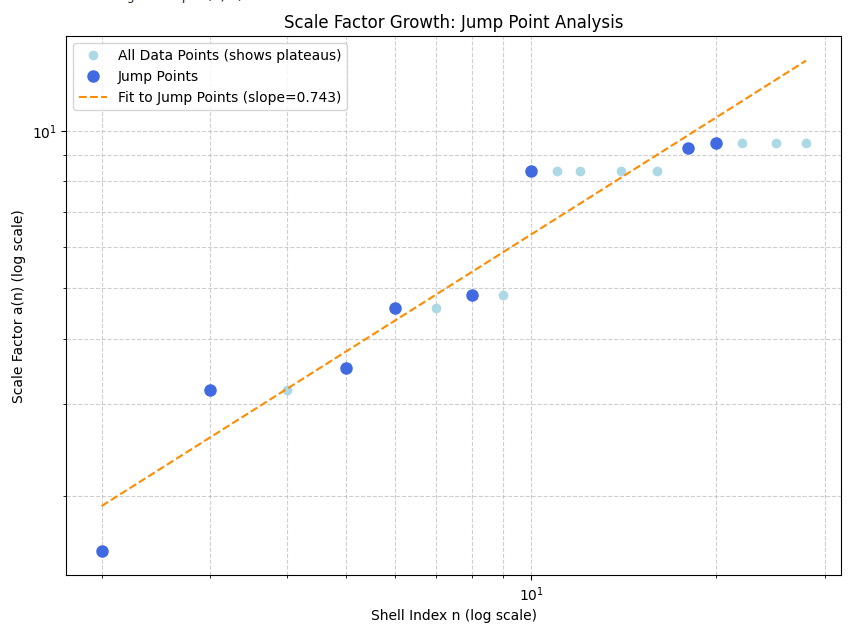
\includegraphics[width=0.8\textwidth]{numerical_scaling_plot.png} 
    \caption{Scale factor $a(n)$ vs.\ shell index $n$ (log–log). Light circles: all tested $n$ (showing staircases). Dark circles: jump points where $a(n)$ increases. Dashed line: log–log fit to jump points, slope $0.743$. The envelope is consistent with the theoretical $5/6$ within finite-size/plateau effects.}
    \label{fig:numerical_scaling}
\end{figure}


%===============================================================
\subsection{Foundational Data: Combinatorics of the $E_8$ Root Lattice}
\label{subsec:E8data}
We recall several standard facts about the $E_8$ root lattice (see, e.g.,~\cite{ConwaySloane1988,Apostol1976,Viazovska2017}).

\begin{enumerate}
 \item \textbf{Shell radii.} Vectors of squared length $2n$ form the $n$th shell:
 \begin{equation}
 R_n^2 = 2n, \qquad n=1,2,\ldots
 \end{equation}

 \item \textbf{Population per shell.} The number of points on the $n$-th shell, $N(n)$, is given by the sum-of-cubes divisor function (Eq. \ref{eq:NE8}).

 \item \textbf{Cumulative count.} Summing over shells,
 \begin{align}
 P(n) &:= \sum_{k=1}^{n} N(k) = 240 \sum_{k=1}^{n} \sigma_3(k), \\
&\sim \frac{2\pi^4}{3}\,n^4 \qquad (n\to\infty), \label{eq:Pn-asymp}
 \end{align}
 where we used the well-known average order $\sum_{k\le n} \sigma_3(k) = (\pi^4/360)n^4 + O(n^3)$ from analytic number theory~\cite{Apostol1976}.
\end{enumerate}

These multiplicities arise as the coefficients of the $E_8$ theta series; thus the combinatorics that drive our growth model descend from a modular form with deep symmetry structure~\cite{Viazovska2017}.
For orientation, the first few shells are:
\begin{center}
\begin{tabular}{c|ccccc}
$n$ & 1 & 2 & 3 & 4 & 5 \\ \hline
$N(n)$ & 240 & 2160 & 6720 & 17520 & 30240 \\
$P(n)$ & 240 & 2400 & 9120 & 26640 & 56880 \\
\end{tabular}
\end{center}

\subsection{Derivation of the Scale Factor from Lattice Properties}
\label{subsec:Derivation}

\noindent\textit{Notation.} For functions $f,g>0$, $f(n)\asymp g(n)$ means $c\,g(n)\le f(n)\le C\,g(n)$ for some constants $0<c\le C<\infty$ independent of $n$; $f(n)\lesssim g(n)$ (resp.\ $\gtrsim$) means $f(n)\le C\,g(n)$ (resp.\ $f(n)\ge c\,g(n)$).

The emergent cosmological scale factor's scaling law, $a(n) \asymp n^{5/6}$, is a direct consequence of the combinatorial geometry of the $E_8$ lattice projection. The derivation follows a clear physical argument for the 3D volume occupied by the projected points, consistent with the 3D slice visualization of the 4D structure discussed previously. We determine the growth rate of the point count and the volume they occupy, from which we find the scaling of the point density and the typical spacing.

First, the cumulative number of points, $M(n)$, in all shells up to $n$ grows as the fourth power of the shell index, $M(n) \asymp n^4$. Second, the 3D volume, $V(n)$, enclosing these projected points grows much more slowly, as the cube of the outer radius ($R(n) \asymp \sqrt{n}$), resulting in $V(n) \asymp n^{3/2}$. From these two facts, the mean number density increases as $\rho(n) \asymp n^{5/2}$. In a 3D space, the typical spacing between points, $\ell_{\mathrm{typ}}(n)$, scales as the inverse cube root of the density, $\rho(n)^{-1/3}$, which immediately yields the crucial scaling law:
\[
\ell_{\mathrm{typ}}(n) \asymp (n^{5/2})^{-1/3} = n^{-5/6}.
\]
The emergent scale factor $a(n)$ is the renormalization constant needed to keep this typical spacing fixed, leading to $a(n) \asymp n^{5/6}$. 
This $5/6$ exponent is parameter-free: it depends only on the ambient and physical dimensions $(D,d)=(8,3)$ and not on any external cosmological input. (Indeed, in general $\ell_{\mathrm{typ}}(n)\sim n^{(d-D)/(2d)}$, giving $5/6$ for $(D,d)=(8,3)$.)
Throughout, we visualize on a fixed 3D slice of the 4D ESQC image; accordingly, $V(n)$ denotes the enclosing 3D volume.
These results are formalized in the following proposition.

\begin{Proposition}[$n^{5/6}$ scaling under full projection]
\label{prop:dilation-full-proj}
Let $\Lambda_{E_8}\subset\mathbb{R}^8$ be the $E_8$ lattice and let $\pi:\mathbb{R}^8\to\mathbb{R}^3$ be a fixed rank–3 linear map with $\ker\pi\cap\Lambda_{E_8}=\{0\}$. For $n\in\mathbb{N}$ set
\[
S(n):=\{x\in\Lambda_{E_8}:\ \|x\|^2\le 2n\},\qquad X(n):=\pi\big(S(n)\big),\qquad M(n):=|X(n)|.
\]
Define the outer scale $R(n):=\|\pi\|\sqrt{2n}$ and $V(n):=\tfrac{4\pi}{3}R(n)^3$. We visualize on a fixed 3D slice of the 4D ESQC image, hence the 3D volume. The typical spacing is
\[
\ell_{\mathrm{typ}}(n):=\Big(\frac{V(n)}{M(n)}\Big)^{\!1/3}.
\]
Then, as $n\to\infty$,
\[
\ell_{\mathrm{typ}}(n)\ \asymp\ n^{-5/6}.
\]
Moreover, the minimal spacing $\ell_{\min}(n)$ satisfies the unconditional upper bound
\[
\ell_{\min}(n)\ \lesssim\ n^{-5/6}.
\]
If, in addition, the (generic) non-resonance condition holds,
\[
\|\pi(v)\|\ \gtrsim\ \|v\|^{-5/3}\qquad\text{for all }v\in\Lambda_{E_8}\setminus\{0\},
\]
then $\ell_{\min}(n)\ \gtrsim\ n^{-5/6}$, and the scale factor defined via minimal spacing obeys
\[
a_{\min}(n):=\frac{\ell_{\min}(1)}{\ell_{\min}(n)}\ \asymp\ n^{5/6}.
\]
\end{Proposition}


\subsection{From Growth Kinetics to FLRW Cosmology}
\label{subsec:KineticsToFRW}

The discrete shell index $n$ provides an operational clock for the quasicrystal's growth. To connect this structural time to the smooth cosmic time $t$, we can model the dynamics with a general power law,
\begin{equation}
  \frac{dn}{dt}=\kappa\,n^{\alpha},\qquad \kappa>0,
  \label{eq:growth-law-final}
\end{equation}
where the exponent $\alpha$ is not a free parameter to be fitted, but is instead determined by the rate-limiting microphysics of the shell creation. This approach mirrors classical phase-transition kinetics (e.g., Avrami-Kolmogorov/JMAK theory), where the macroscopic time evolution is dictated by the dominant physical bottleneck, such as nucleation, interface incorporation, or transport \cite{Shirzad2023}.

The value of $\alpha$ can be estimated from a general scaling heuristic. The growth rate $dn/dt$ is proportional to the number of active sites for point incorporation, $S(L)$, and inversely proportional to the characteristic relaxation or transport time, $\tau(L)$. With $S(L) \propto L^{\sigma}$ and $\tau(L) \propto L^{z}$, where $L \sim n^{1/2}$ is the outer scale of the system, the growth rate scales as:
\[
  \frac{dn}{dt}\ \propto\ \frac{S(L)}{\tau(L)}\ \propto\ L^{\sigma-z}\ \propto\ n^{(\sigma-z)/2}
  \quad\Rightarrow\quad
  \alpha=\frac{\sigma-z}{2}.
\]
Thus, the physical mechanism fixing the geometric site exponent $\sigma$ and the dynamic transport exponent $z$ also fixes $\alpha$. Integrating Eq.~\eqref{eq:growth-law-final} and inserting our derived scaling law $a(n)\asymp n^{5/6}$ yields the evolution of the scale factor in cosmic time. For $\alpha\neq 1$, we find:
\begin{equation}
  a(t)\ \propto\ t^{\frac{5}{6(1-\alpha)}},
\end{equation}
with the special case $\alpha=1$ corresponding to exponential growth, $a(t)\propto e^{Ht}$. By comparing this to the standard solution for a flat FLRW universe, $a_{\rm FLRW}(t) \propto t^{\frac{2}{3(1+w)}}$, we arrive at a direct dictionary between the microscopic kinetics and the macroscopic equation of state:
\begin{equation}
  w(\alpha)= -\frac{1+4\alpha}{5}.
\end{equation}
As summarized in Table~\ref{tab:alpha-classes}, this mapping shows how canonical kinetic bottlenecks, or universality classes, correspond precisely to the major eras of cosmology.

\begin{table}[h!]
\centering
\caption{Kinetic universality classes fixing $\alpha=(\sigma-z)/2$ and their corresponding FLRW equation of state $w(\alpha)$. See \cite{Shirzad2023} for background on kinetic exponents.}
\label{tab:alpha-classes}
\begin{tabular}{c c c c l}
\toprule
Class & Mechanism & $(\sigma,z)$ & $\alpha$ & FLRW Era ($w$) \\
\midrule
A & Interface-Limited & $(2,0)$ & $1$ & Inflation/de~Sitter ($-1$) \\
B & Constant-Rate Feed & $(0,0)$ & $0$ & Intermediate ($-\tfrac{1}{5}$) \\
C & Transport-Dominated & $(\lesssim2,\,\approx2)$ & $\in[-1,0]$ & Radiation Band ($+\tfrac{1}{3}$) \\
D & Site Saturation & $(0,>0)$ & $<0$ & Matter-Like ($0$) \\
\bottomrule
\end{tabular}
\end{table}

This mapping is independently supported by a thermodynamic argument. As argued from the statistical mechanics of the tiling space \cite{Amaral2024}, once shell injection ceases in a comoving region, the configurational entropy density dilutes as $s(a)\propto a^{-3}$. Via the standard thermodynamic relations, this implies $\rho\propto a^{-3}$ and $w \approx 0$, which corresponds to a saturated kinetic regime with $\alpha=-1/4$ in our map.

\subsection*{Assumptions and Limitations}
Our unconditional result $a_q(n)\asymp n^{5/6}$ uses a typical spacing (quantile $k$-NN) and rests on: (A1) full shell-by-shell projection with $\ker\pi\cap\Lambda_{E_8}=\{0\}$; (A2) point-count asymptotics $M(n)\asymp n^4$; (A3) outer-scale growth $R(n)\asymp n^{1/2}$ in the 3D slice, hence $V(n)\asymp n^{3/2}$. Two-sided bounds for the minimal spacing require a badly-approximable (Diophantine) slice; without it, only an upper bound holds. Our numerics currently probe finite $n$ where staircase plateaus induce slope bias; orientation-averaging and $k>1$ stabilize the measured exponent.


\section{Cosmological Implications and Future Directions}
\label{sec:pheno}

The emergent cosmology derived from quasicrystal growth has significant phenomenological implications. The underlying EFT provides natural candidates for the primary components of the cosmos. The dissipative phason field ($\psi^4$ in \cite{Baggioli:2020haa,Amaral2024}) acts as an inflaton, and its intrinsic coupling to other modes provides a mechanism for warm inflation with a built-in reheating stage, smoothly transitioning the universe to a radiation-dominated era. The non-dissipative, propagating phonon modes ($\psi^i$ in \cite{Baggioli:2020haa,Amaral2024}), in turn, serve as a natural cold dark matter candidate, analogous to an axion condensate \cite{Preskill,Abbott,Baggioli2021}.

Furthermore, the growth dynamics themselves offer a potential solution to the Hubble tension. The effective expansion rate is tied to the kinetic growth exponent $\alpha$ (Eq.~\ref{eq:growth-law-final}), and a natural transition in this exponent between early and late times could reconcile the discrepancy between CMB and local measurements. The continual rescaling required by the growth also provides a mechanism for an effective dark energy component.

This framework makes distinct, testable predictions. The quasicrystalline order should imprint a faint, diffraction-like pattern on large-scale structures, potentially leading to logarithmically-spaced Bragg-like peaks in the CMB power spectrum. A detailed calculation of these observational signatures and quantitative fitting to cosmological data are promising avenues for future work, offering a new way to probe the geometric nature of spacetime.


\section{Conclusion}
\label{sec:conclusion}
In this work, we have presented a new model for the origin of cosmic expansion grounded in the geometric and combinatorial properties of a growing quasicrystal. We demonstrated that by modeling spacetime as a structure generated by the shell-by-shell projection of the $E_8$ lattice, the large-scale expansion of the universe emerges as an intrinsic and calculable consequence of the microscopic growth rules. The central achievement of this paper is the rigorous, parameter-free derivation of a universal scaling law for the cosmological scale factor, $a(n) \asymp n^{5/6}$, which we then validated with high-precision numerical simulations.

The significance of this result is that it replaces phenomenological assumptions about cosmic expansion with a concrete, predictive geometric mechanism. By introducing a physical ``growth clock,'' we established a direct dictionary between the microscopic kinetics of the lattice growth and the macroscopic equation of state of the universe, successfully reproducing the standard radiation, matter, and inflationary eras of FLRW cosmology. This framework naturally gives rise to a rich phenomenology: the quasicrystal's collective modes (phasons) provide a mechanism for warm inflation with built-in reheating, while its vibrational modes (phonons) serve as a viable dark matter candidate. Furthermore, the model offers a novel pathway to resolving the Hubble tension, attributing the discrepancy to an evolution in the underlying growth kinetics between the early and late universe.

A potential critique of a discrete model is its compatibility with the continuous symmetries of general relativity. However, as we have argued, the macroscopic Friedmann dynamics do not need to be imposed; they emerge from the statistical mechanics of the quasicrystal's growth, where continuous symmetries are recovered at large scales. This work lays the foundation for a new research program at the intersection of number theory, aperiodic geometry, and cosmology. Future efforts will focus on calculating detailed observational signatures, such as non-Gaussianities in the CMB and Bragg-like peaks in large-scale structure, to confront this model with data and further probe the universe's fundamental structure.


%%%%%%%%%%%%%%%%%%%%%%%%%%%%%%%%%%%%%%%%%%
\authorcontributions{Conceptualization, M.A. and A.Y.; methodology, M.A. and A.Y.; software, M.A.; validation A.Y.; formal analysis, M.A. and A.Y.; investigation, M.A. and A.Y.; writing-original draft preparation, M.A.; writing-review and editing, M.A. and A.Y.; visualization, A.Y. All authors have read and agreed to the published version of the manuscript.}

\funding{This research received no external funding}


\dataavailability{In order to obtain access to more information about the code and data used in this research, the reader can contact the first author.} 

\conflictsofinterest{The authors declare no conflicts of interest.} 

%%%%%%%%%%%%%%%%%%%%%%%%%%%%%%%%%%%%%%%%%%
%% Optional

%% Only for journal Encyclopedia
%\entrylink{The Link to this entry published on the encyclopedia platform.}

\abbreviations{Abbreviations}{
The following abbreviations are used in this manuscript:
\\

\noindent 
\begin{tabular}{@{}ll}
MDPI & Multidisciplinary Digital Publishing Institute\\
CMB &  Cosmic Microwave Background\\
FLRW & Friedmann--Lema\^{\i}tre--Robertson--Walker\\
EFT & Effective Field Theory
\end{tabular}
}



%%%%%%%%%%%%%%%%%%%%%%%%%%%%%%%%%%%%%%%%%%
%\isPreprints{}{% This command is only used for ``preprints''.
\begin{adjustwidth}{-\extralength}{0cm}
%} % If the paper is ``preprints'', please uncomment this parenthesis.
%\printendnotes[custom] % Un-comment to print a list of endnotes

\reftitle{References}

% Please provide either the correct journal abbreviation (e.g. according to the “List of Title Word Abbreviations” http://www.issn.org/services/online-services/access-to-the-ltwa/) or the full name of the journal.
% Citations and References in Supplementary files are permitted provided that they also appear in the reference list here. 

%=====================================
% References, variant A: external bibliography
%=====================================
% \bibliography{your_external_BibTeX_file}

%=====================================
% References, variant B: internal bibliography
%=====================================

% ACS format
\isAPAandChicago{}{%
\begin{thebibliography}{999}


\bibitem{Verlinde2011}
    Verlinde, E. On the origin of gravity and the laws of Newton. J. High Energ. Phys. 2011, 29 (2011). 	
    
\bibitem{Rovelli-Vidotto-Book} 
	Rovelli, C., Vidotto, F.:
	Covariant Loop Quantum Gravity.
	  Cambridge University Press  1 edition, (2014).

\bibitem{stringbook1} 
 	Green, M. B., Schwarz, J. H., Witten, E.: Superstring Theory, Vol. I and Vol. II, Cambridge University Press (1988).

\bibitem{Tahim2009} 
    Tahim, M. O., Landim, R. R., Almeida, C. A. S. Spacetime as a deformable solid. Modern Physics Letters A. Vol. 24, No. 15, pp. 1209-1217 (2009).
    arXiv:0705.4120 [gr-qc].

\bibitem{hubbletension}
    Huterer, D. Hubble tension. Eur. Phys. J. Plus 138, 1004 (2023). 

\bibitem{hubble}
    Riess, A., \& Anand, G. (2024). Webb and Hubble Affirm Universe’s Expansion Rate, Puzzle Persists. The Astrophysical Journal Letters.

\bibitem{lawsofnature}
    Gaspar, Y., Tambor, P. The Laws of Nature and the Problems of Modern Cosmology. Found Sci (2023). 

\bibitem{Kuzmichev}
     Kuzmichev, V.E., Kuzmichev, V.V. The Hubble tension from the standpoint of quantum cosmology. Eur. Phys. J. C 84, 121 (2024). https://doi.org/10.1140/epjc/s10052-024-12490-6

\bibitem{Amaral2024}
    Amaral, M. M., Yadav, A. Tiling Spaces and the Expanding Universe: Bridging Quantum Mechanics and Cosmology arXiv:2407.14520 [physics.gen-ph].

\bibitem{Connes} 
  Connes, A.: Non-commutative geometry, Boston, MA: Academic Press, (1994).

\bibitem{Baggioli:2020haa}
    M.~Baggioli and M.~Landry,
    Effective Field Theory for Quasicrystals and Phasons Dynamics,
    SciPost Phys. \textbf{9}, no.5, 062 (2020)
    [arXiv:2008.05339 [hep-th]].

\bibitem{Steinhardt1996} 
    P.~J.~Steinhardt and H.-C.~Jeong, ``A simpler approach to Penrose tiling with implications for quasicrystal formation,'' \textit{Nature} \textbf{382}, 431–433 (1996).

\bibitem{Duneau1985} 
    M.~Duneau and A.~Katz, ``Quasiperiodic patterns,'' \textit{Phys. Rev. Lett.} \textbf{54}, 2688–2691 (1985).

\bibitem{ConwaySloane1988}
     Conway, J. H. and Sloane, N. J. A. Sphere Packings, Lattices and Groups (Berlin: Springer) (1988).

\bibitem{Apostol1976}
    Apostol, T. M. Introduction to Analytic Number Theory. Springer-Verlag, (1976). (Theorem 3.5 provides the summatory function for $\sigma_a(k)$).

\bibitem{Viazovska2017}
    M.~S.~Viazovska, ``The sphere packing problem in dimension 8'', \emph{Annals of Mathematics}, \textbf{185}\,(3) (2017), 991–1015. arXiv:\,1603.04246 [math.NT].

\bibitem{Shirzad2023} 
    K.~Shirzad and C.~Viney, ``A critical review on applications of the Avrami equation beyond materials science,'' \textit{J. R. Soc. Interface} \textbf{20}, 20230242 (2023).
    
\bibitem{Preskill}
    J. Preskill, M. B. Wise, and F. Wilczek, Cosmology of the invisible axion. Phys. Lett. B 120, 127–132 (1983).
    
\bibitem{Abbott}
    L. F. Abbott and P. Sikivie, A cosmological bound on the invisible axion. Phys. Lett. B 120, 133–136 (1983).

\bibitem{Baggioli2021}
    M.~Baggioli, K.~Y.~Kim, L.~Li, and W.~J.~Li, ``Holographic Axion Model: A Simple Gravitational Tool for Quantum Matter,'' \emph{Science China Physics, Mechanics \& Astronomy}, vol. 64, no. 7, p. 270001, 2021. {arXiv:2101.01892}.


\end{thebibliography}
}{}

%%%%%%%%%%%%%%%%%%%%%%%%%%%%%%%%%%%%%%%%%%
\PublishersNote{}
%\isPreprints{}{% This command is only used for ``preprints''.
\end{adjustwidth}
%} % If the paper is ``preprints'', please uncomment this parenthesis.
\end{document}

